\documentclass[11pt]{article}
\usepackage{graphicx}
\usepackage{listings}
\usepackage[margin=1in]{geometry}
\usepackage{placeins}
\usepackage{float}
\lstset{language=python}

\author{Andrew Smith, Kofi Otseidu, Manav Trivedi}
\title{Visualization}

\begin{document}
\maketitle

\section{Allegations Per Capita in Chicago Neighborhoods}
This and the next question use a simple SQL query to extract the data needed. It did, however take a bit of effort to get the data in a Tableau usable format, particularly for the geographic data. We ended up using python and geopandas to create a GeoJSON which Tableau would understand.

The allegations per capita is similar across the board, with a few neighborhoods standing out. First and foremost is Fuller Park, the only neighborhood in red in the first map, as it has almost as many complaints as residents (around 2,000).

\begin{figure}[h]
\centering
\caption{Allegations per Capita}
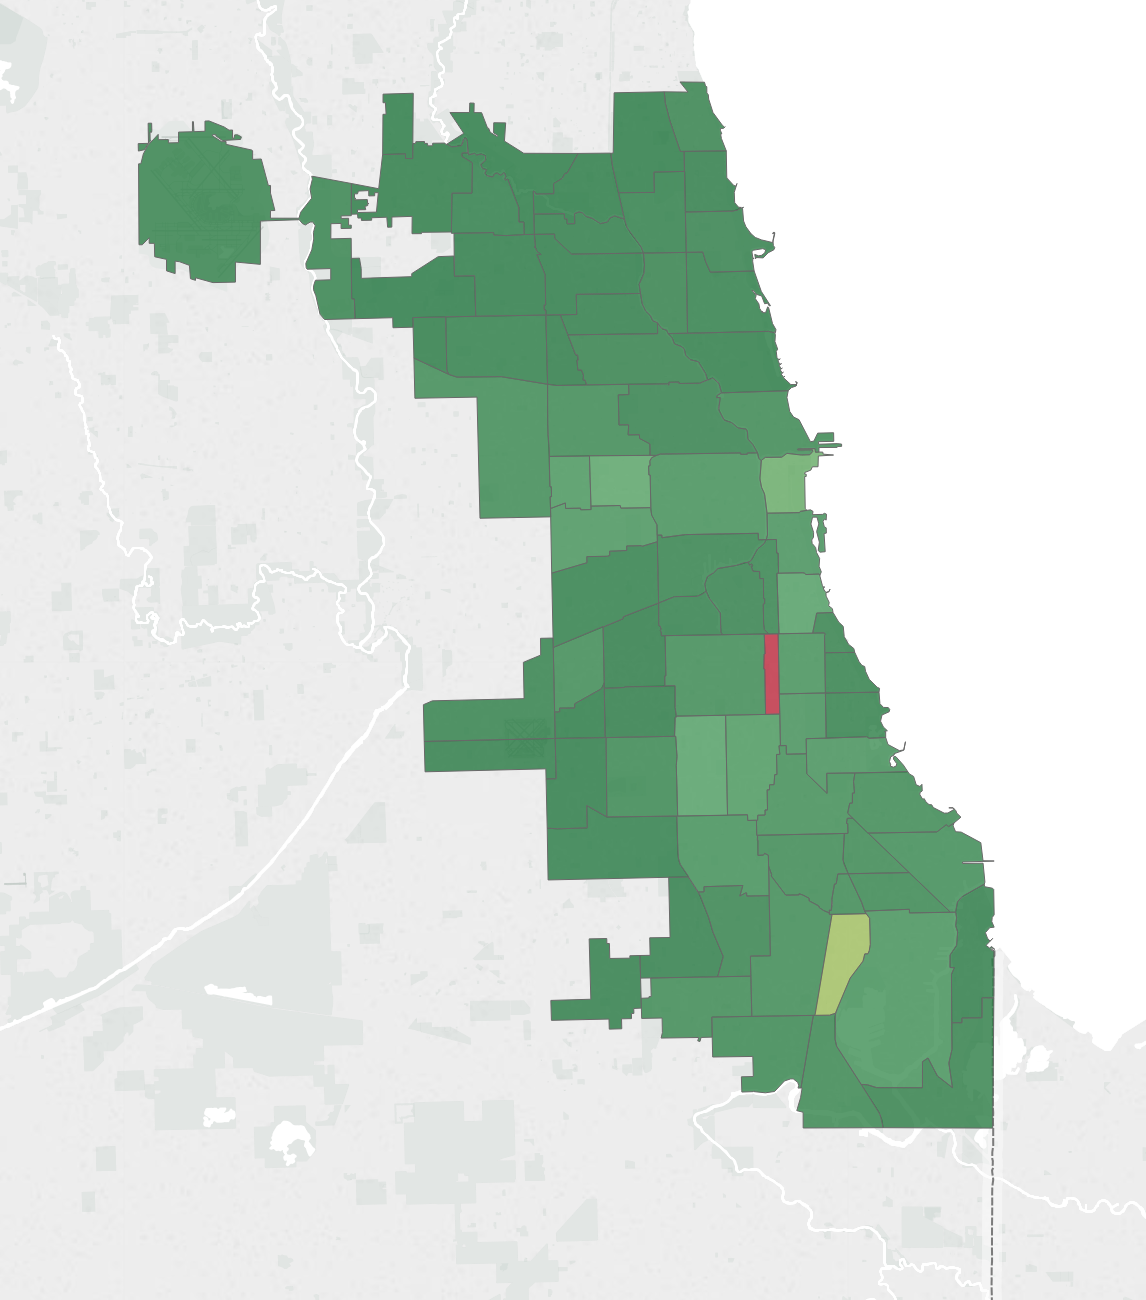
\includegraphics[width=0.5\textwidth]{plot1.png}
\end{figure}

Excluding Fuller Park we can see that a few other neighborhoods have elevated complaint levels, namely the Loop and a few west and south side areas. The Loop has lots of traffic, and the other neighborhood are rougher areas, so it makes sense that they have more complaints per capita.

\begin{figure}[h]
\centering
\caption{Allegations per Capita (excluding Fuller Park}
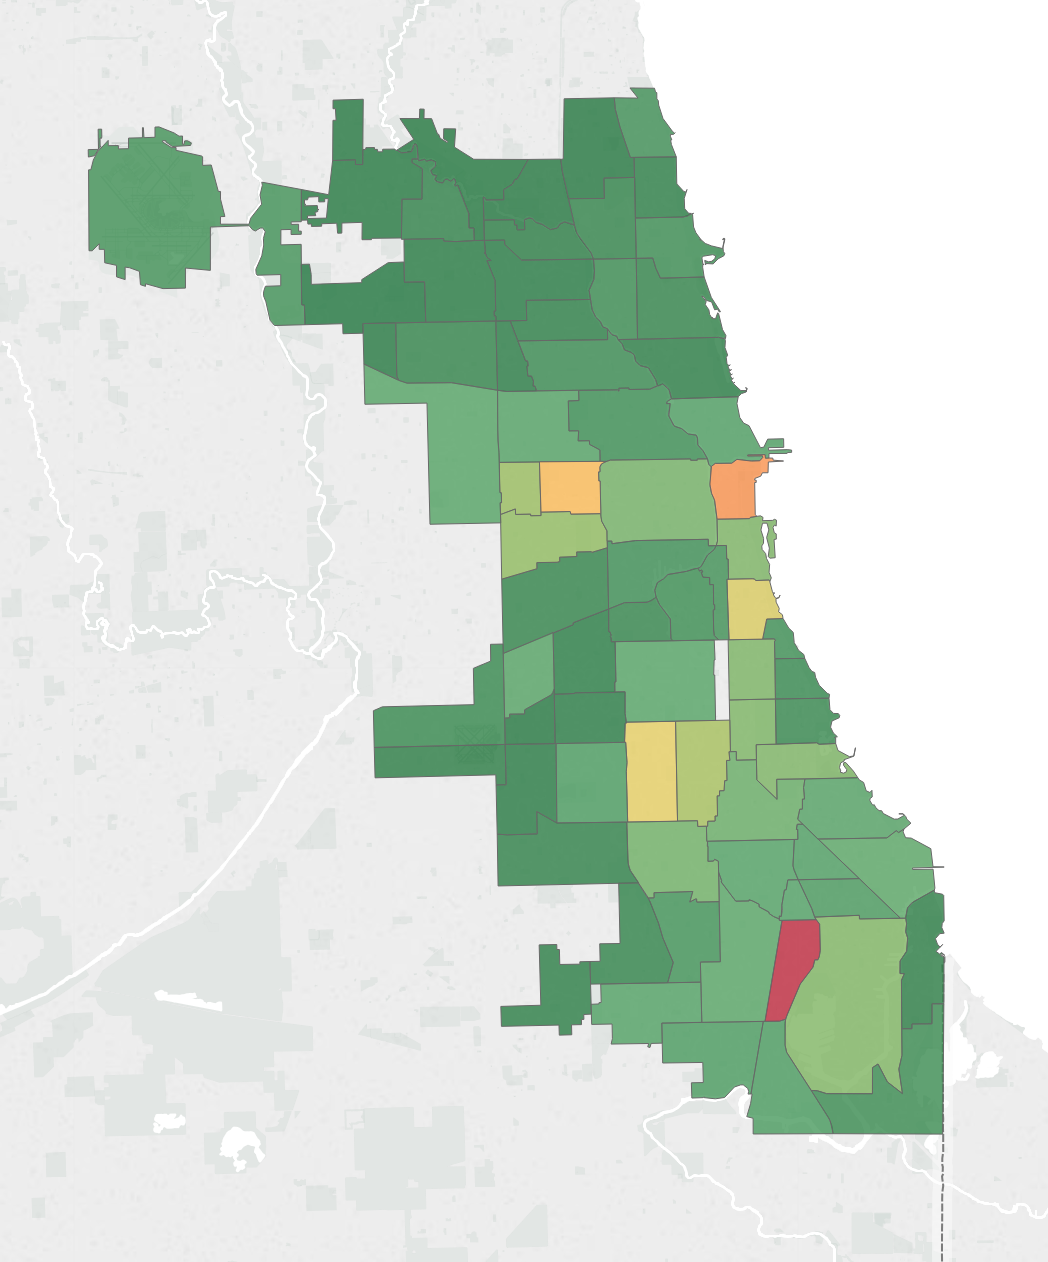
\includegraphics[width=0.5\textwidth]{plot2.png}
\end{figure}

\FloatBarrier

\section{Median Income per Neighborhood}
This plot is pretty similar to the number of settlements per neighborhood plot we made in an earlier checkpoint. There are a few outliers, the Loop and Austin, and presumably some spillover from the Loop in the Near West and Near North Side. Excluding those, it looks like generally, the number of complaints is inversely correlated with median income. There are some neighborhood with low incomes that also don't report many complaints. It's possible these neighborhoods don't believe the police will help and are thus under reported, but it would be hard to prove this without further analysis. In addition, neighborhoods such as the Loop and Near West Side may over report for allegations for many things that may not really classify as allegation due to the nature of these wealthier areas. However more analysis on the types of analysis done would be required.

\begin{figure}[h]
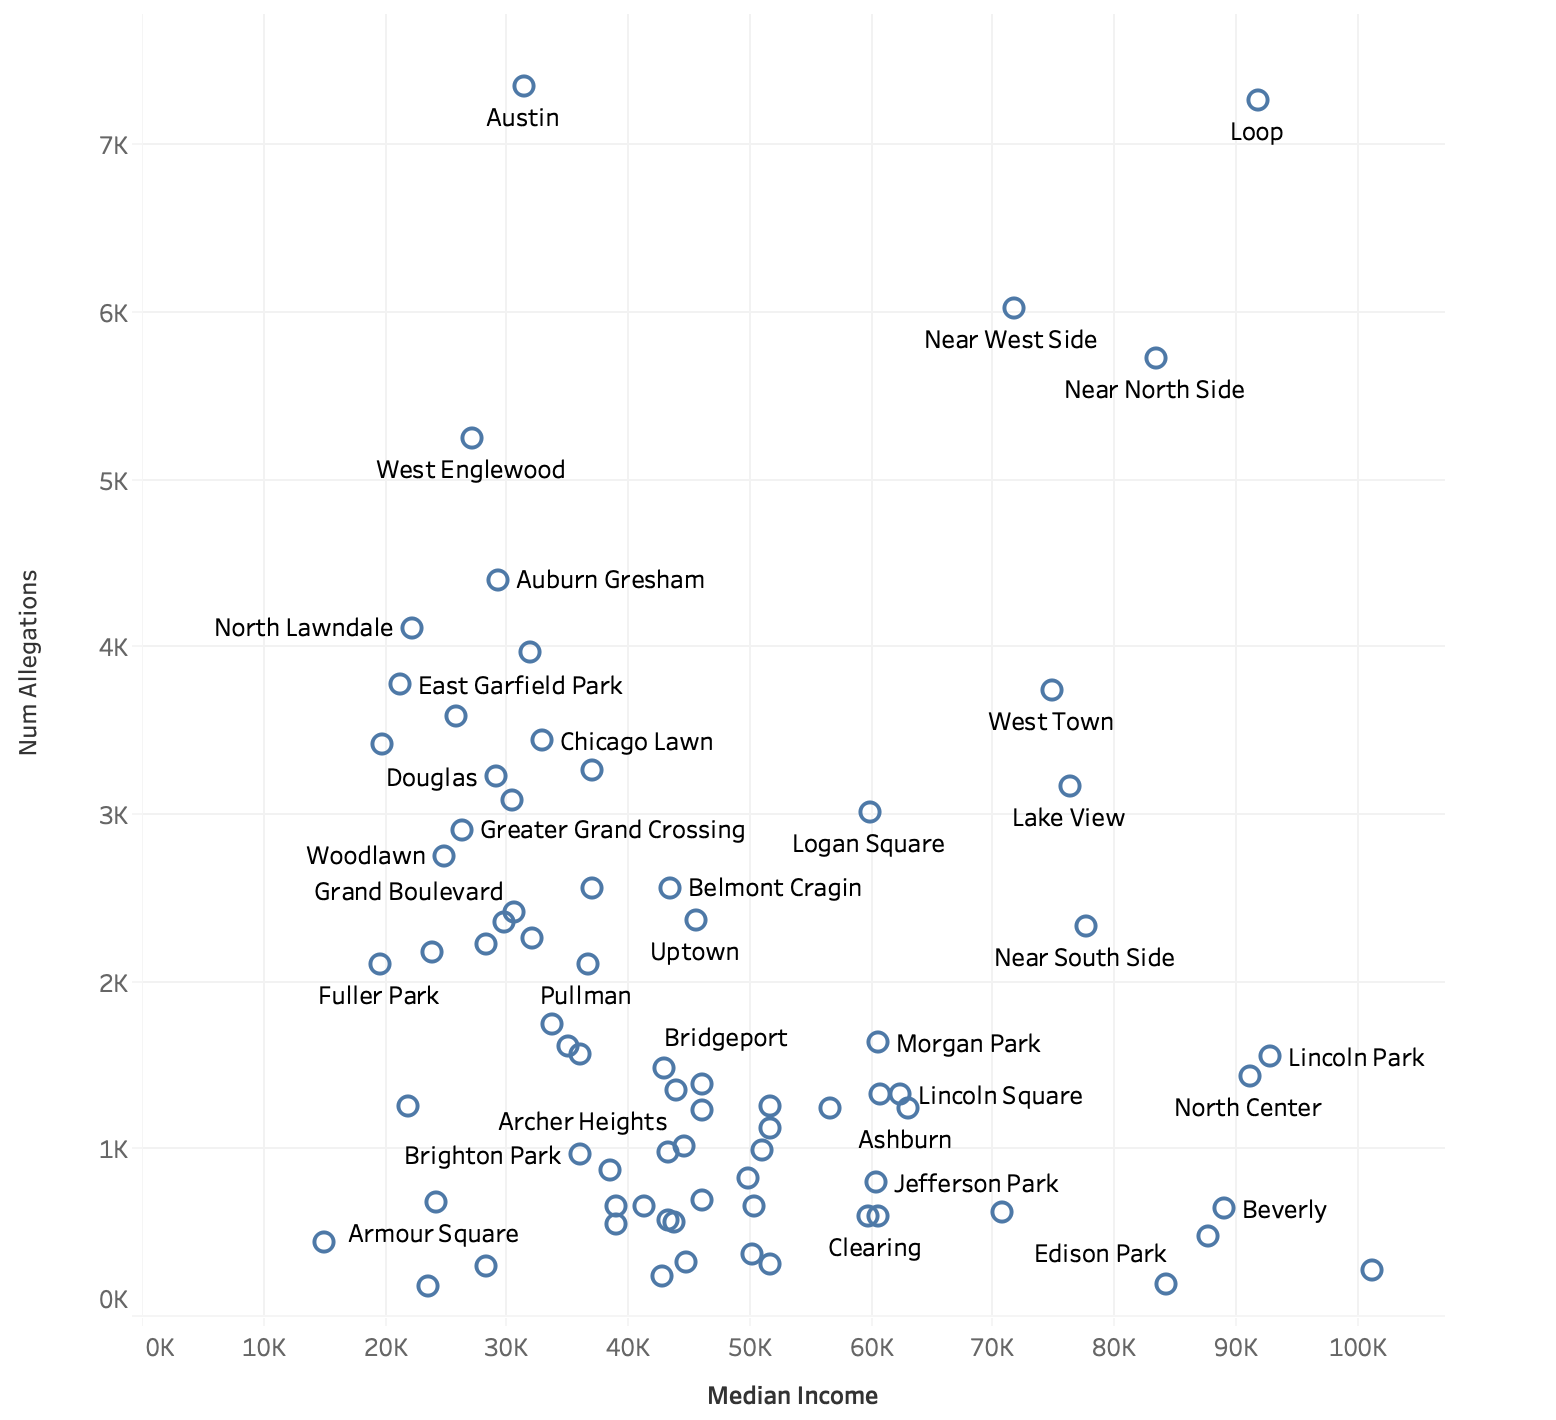
\includegraphics[width=\textwidth]{scatter.png}
\end{figure}

\FloatBarrier

\section{Cost of Officers Over Time}
It was pretty tricky to get the data formatted for this, but essentially I used the salary table to create a listing of salary for each year for each officer. The table however, doesn't seem to include values if the officer's pay does not change, so I had to write a short python script to fill in those values. From there I also included the cost of any settlements incurred by the officer in their 'salary' for that year. I made sure to divy up the cost of the settlement to each officer involved. Then I counted the number of allegations for each officer (over all time) and grouped the officers into quartiles by number of allegations. This creates the plot below.

\begin{figure}[h]
\caption{Cost of Officers from 2002-2017}
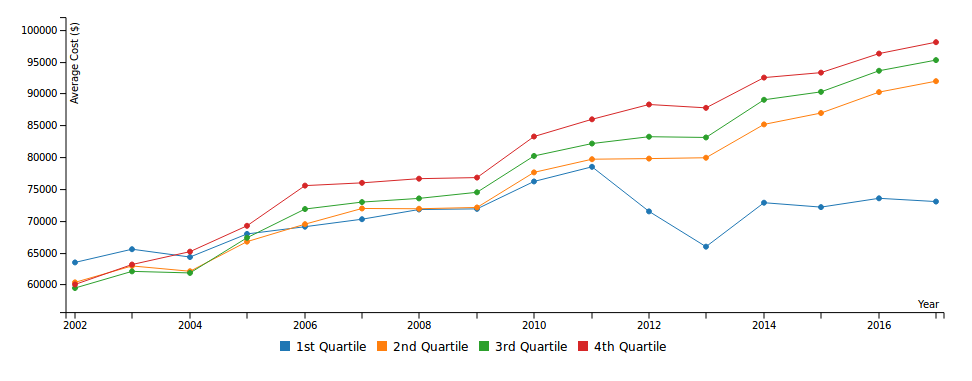
\includegraphics[width=\textwidth]{costline.png}
\end{figure}

The first thing that stands out is how much the average is increasing year to year. It seems to be a much larger increase than just inflation so I'm not entirely sure what is causing it. It does show that the officers with more complaints generally cost more, although I don't think the settlements are factoring into the average very much. It mostly comes down to more senior officers having more complaints and also a higher salary, both because they simply have been on the force longer. There is also a huge dip in the first quartile officers, that is due to the fact that many new officers were hired in the last few years.

The first quartile consist of officer who have two complaints or less, with an average of 0.64 complaints. The second quartile is officer with 2 to 7 complaints, with an average of 4.94. The third quartile is officers with 7 to 15 complaints, with an average of 11, and the last quartile has up to 175 complaints, with an average of 27.9 complaints per officer.

I'm not entirely sure we wouldn't get somewhat better results if we calculated quartiles for each year as opposed to overall quartiles, but I don't think it would change much and the increasing average would still be present.

\end{document}